% Editable vector schematic of completed observed-CE raw25 factorial.
% Sources: modal_encoder_chemistry_input_effects.py and committed
% input_metadata_factorial manifests. This is not a molecule or spectrum edit.
\documentclass[tikz,border=0pt]{standalone}
\usepackage{fontspec}
\setsansfont{LiberationSans}[Path=../../shared/assets/,Extension=.ttf,UprightFont=*-Regular,BoldFont=*-Bold]
\usepackage{amsmath}
\usepackage{unicode-math}
\setmathfont{Latin Modern Math}
\usetikzlibrary{arrows.meta,calc}
\definecolor{ink}{HTML}{0C0C0C}
\definecolor{muted}{HTML}{63676B}
\definecolor{accent}{HTML}{007C83}
\definecolor{control}{HTML}{A36F23}
\definecolor{lightfill}{HTML}{EDF6F5}
\hyphenpenalty=10000\exhyphenpenalty=10000
\begin{document}
\ifdefined\SlideDiagram
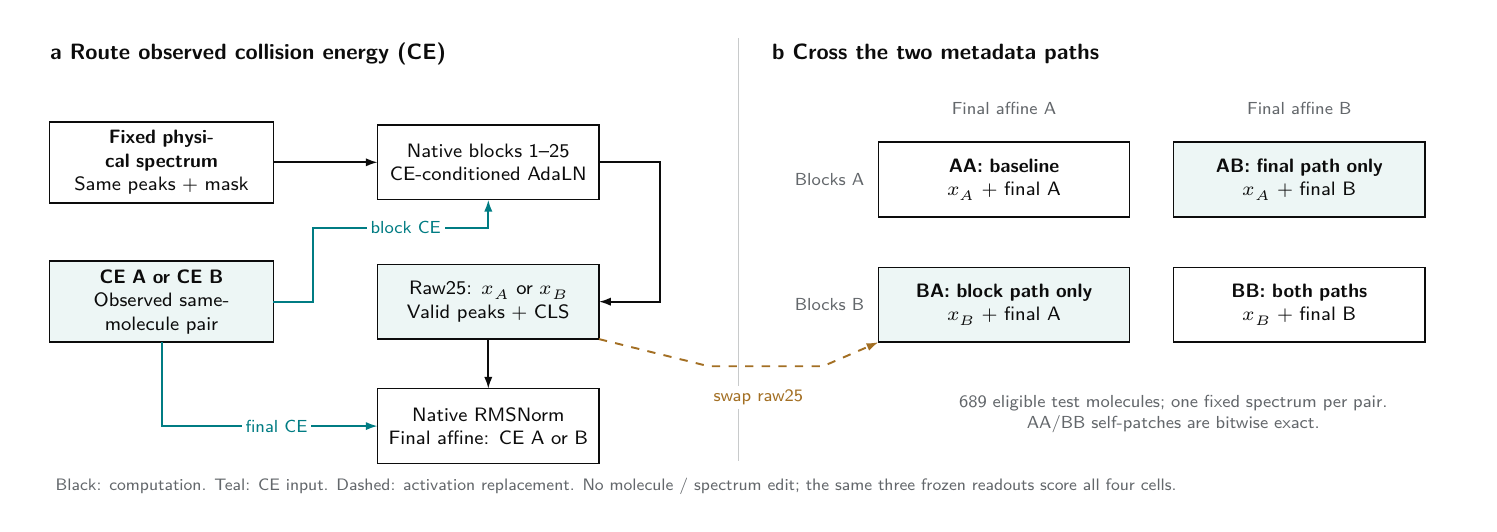
\begin{tikzpicture}[x=1cm,y=1cm,
 every node/.style={font=\sffamily\fontsize{7}{8.5}\selectfont,text=ink,align=center,inner sep=3pt,outer sep=0pt},
 box/.style={draw=ink,line width=.55pt,minimum height=.95cm},
 flow/.style={-{Latex[length=1.5mm,width=1.05mm]},line width=.65pt,draw=ink},
 context/.style={-{Latex[length=1.5mm,width=1.05mm]},line width=.7pt,draw=accent},
 patch/.style={-{Latex[length=1.5mm,width=1.05mm]},line width=.7pt,draw=control,dashed},
 note/.style={font=\sffamily\fontsize{6.3}{7.6}\selectfont,text=muted},
 panel/.style={anchor=west,font=\sffamily\bfseries\fontsize{8}{10}\selectfont}]
\path[use as bounding box] (0,0) rectangle (18.3,6.05);
\node[panel] at (.18,5.72) {a  Route observed collision energy (CE)};
\node[panel] at (9.35,5.72) {b  Cross the two metadata paths};
\draw[muted!35,line width=.4pt] (9.03,.55)--(9.03,5.92);
\node[box,text width=2.63cm] (sp) at (1.7,4.34)
 {\textbf{Fixed physical spectrum}\\Same peaks + mask};
\node[box,text width=2.6cm] (sb) at (5.85,4.34)
 {Native blocks 1--25\\CE-conditioned AdaLN};
\draw[flow] (sp.east)--(sb.west);
\node[box,text width=2.63cm,fill=lightfill] (sce) at (1.7,2.57)
 {\textbf{CE A or CE B}\\Observed same-molecule pair};
\node[box,text width=2.6cm,fill=lightfill] (sx) at (5.85,2.57)
 {Raw25: $x_A$ or $x_B$\\Valid peaks + CLS};
\draw[context] (sce.east)--(3.62,2.57)--(3.62,3.51)--(5.85,3.51)--(sb.south);
\node[note,text=accent,fill=white,inner sep=1.4pt] at (4.8,3.51) {block CE};
\draw[flow] (sb.east)--(8.03,4.34)--(8.03,2.57)--(sx.east);
\node[box,text width=2.6cm] (sf) at (5.85,.99)
 {Native RMSNorm\\Final affine: CE A or B};
\draw[flow] (sx.south)--(sf.north);
\draw[context] (sce.south)--(1.7,.99)--(sf.west);
\node[note,text=accent,fill=white,inner sep=1.4pt] at (3.16,.99) {final CE};
\node[note] at (12.4,5.03) {Final affine A};
\node[note] at (16.15,5.03) {Final affine B};
\node[anchor=east,note] at (10.73,4.12) {Blocks A};
\node[anchor=east,note] at (10.73,2.53) {Blocks B};
\node[box,text width=2.98cm] (saa) at (12.4,4.12)
 {\textbf{AA: baseline}\\$x_A$ + final A};
\node[box,text width=2.98cm,fill=lightfill] (sab) at (16.15,4.12)
 {\textbf{AB: final path only}\\$x_A$ + final B};
\node[box,text width=2.98cm,fill=lightfill] (sba) at (12.4,2.53)
 {\textbf{BA: block path only}\\$x_B$ + final A};
\node[box,text width=2.98cm] (sbb) at (16.15,2.53)
 {\textbf{BB: both paths}\\$x_B$ + final B};
\draw[patch] (sx.south east)--(8.65,1.75)--(10.1,1.75)--(sba.south west);
\node[note,text=control,fill=white,inner sep=1.4pt] at (9.28,1.35) {swap raw25};
\node[note,text width=6.1cm] at (14.55,1.14)
 {689 eligible test molecules; one fixed spectrum per pair.\\AA/BB self-patches are bitwise exact.};
\node[anchor=west,note,font=\sffamily\fontsize{6}{7.2}\selectfont] at (.25,.23)
 {Black: computation. Teal: CE input. Dashed: activation replacement. No molecule / spectrum edit; the same three frozen readouts score all four cells.};
\end{tikzpicture}
\else
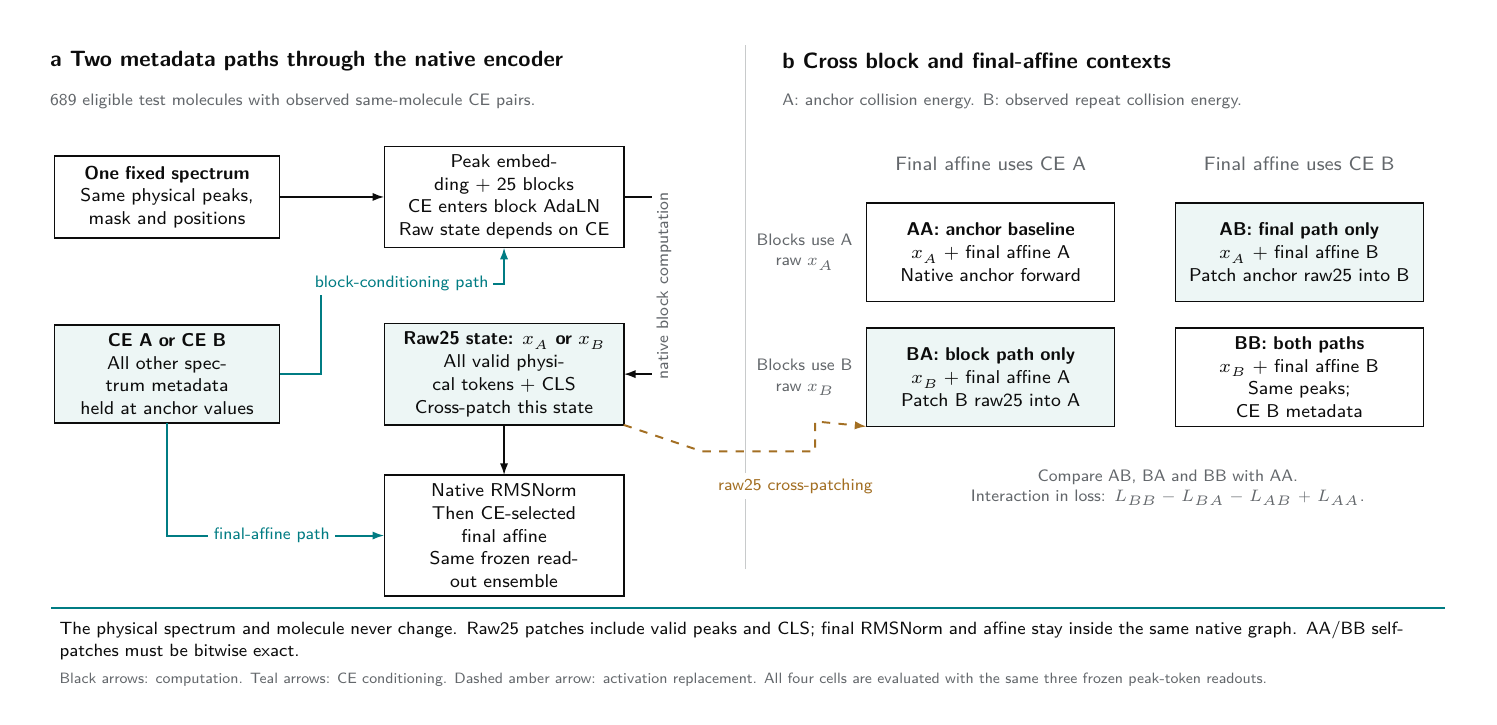
\begin{tikzpicture}[x=1cm,y=1cm,
 every node/.style={font=\sffamily\fontsize{6.7}{8.2}\selectfont,text=ink,align=center,inner sep=3pt,outer sep=0pt},
 box/.style={draw=ink,line width=.55pt,minimum height=1.04cm},
 flow/.style={-{Latex[length=1.5mm,width=1.05mm]},line width=.65pt,draw=ink},
 context/.style={-{Latex[length=1.5mm,width=1.05mm]},line width=.7pt,draw=accent},
 patch/.style={-{Latex[length=1.5mm,width=1.05mm]},line width=.7pt,draw=control,dashed},
 note/.style={font=\sffamily\fontsize{6}{7.4}\selectfont,text=muted},
 panel/.style={anchor=west,font=\sffamily\bfseries\fontsize{8}{10}\selectfont}]
\path[use as bounding box] (0,0) rectangle (18.3,8.5);
\node[panel] at (.18,8.08) {a  Two metadata paths through the native encoder};
\node[panel] at (9.48,8.08) {b  Cross block and final-affine contexts};
\node[note,anchor=west] at (.18,7.56) {689 eligible test molecules with observed same-molecule CE pairs.};
\node[note,anchor=west] at (9.48,7.56) {A: anchor collision energy. B: observed repeat collision energy.};
\draw[muted!35,line width=.4pt] (9.12,1.62)--(9.12,8.28);

\node[box,text width=2.65cm] (spectrum) at (1.77,6.35)
 {\textbf{One fixed spectrum}\\Same physical peaks,\\mask and positions};
\node[box,text width=2.83cm] (blocks) at (6.05,6.35)
 {Peak embedding + 25 blocks\\CE enters block AdaLN\\Raw state depends on CE};
\draw[flow] (spectrum.east)--(blocks.west);
\node[box,text width=2.65cm,fill=lightfill] (ce) at (1.77,4.1)
 {\textbf{CE A or CE B}\\All other spectrum metadata\\held at anchor values};
\draw[context] (ce.east)--(3.72,4.1)--(3.72,5.25)--(6.05,5.25)--(blocks.south);
\node[note,text=accent,fill=white,inner sep=1.5pt] at (4.75,5.25) {block-conditioning path};
\node[box,text width=2.83cm,fill=lightfill] (raw) at (6.05,4.1)
 {\textbf{Raw25 state: $x_A$ or $x_B$}\\All valid physical tokens + CLS\\Cross-patch this state};
\draw[flow] (blocks.east)--(8.08,6.35)--(8.08,4.1)--(raw.east);
\node[note,rotate=90,fill=white,inner sep=1.5pt] at (8.08,5.22) {native block computation};
\node[box,text width=2.83cm] (final) at (6.05,2.05)
 {Native RMSNorm\\Then CE-selected final affine\\Same frozen readout ensemble};
\draw[flow] (raw.south)--(final.north);
\draw[context] (ce.south)--(1.77,2.05)--(final.west);
\node[note,text=accent,fill=white,inner sep=2pt] at (3.1,2.05) {final-affine path};

\node[note,font=\sffamily\fontsize{7}{8.5}\selectfont] at (12.23,6.77) {Final affine uses CE A};
\node[note,font=\sffamily\fontsize{7}{8.5}\selectfont] at (16.15,6.77) {Final affine uses CE B};
\node[anchor=east,note] at (10.58,5.65) {Blocks use A\\raw $x_A$};
\node[anchor=east,note] at (10.58,4.06) {Blocks use B\\raw $x_B$};
\node[box,text width=2.94cm,minimum height=1.25cm] (aa) at (12.23,5.65)
 {\textbf{AA: anchor baseline}\\$x_A$ + final affine A\\Native anchor forward};
\node[box,text width=2.94cm,minimum height=1.25cm,fill=lightfill] (ab) at (16.15,5.65)
 {\textbf{AB: final path only}\\$x_A$ + final affine B\\Patch anchor raw25 into B};
\node[box,text width=2.94cm,minimum height=1.25cm,fill=lightfill] (ba) at (12.23,4.06)
 {\textbf{BA: block path only}\\$x_B$ + final affine A\\Patch B raw25 into A};
\node[box,text width=2.94cm,minimum height=1.25cm] (bb) at (16.15,4.06)
 {\textbf{BB: both paths}\\$x_B$ + final affine B\\Same peaks; CE B metadata};
\draw[patch] (raw.south east)--(8.56,3.12)--(10.0,3.12)--(10.0,3.5)--(ba.south west);
\node[note,text=control,fill=white,inner sep=2pt] at (9.75,2.68) {raw25 cross-patching};
\node[note,text width=6.1cm] at (14.48,2.66)
 {Compare AB, BA and BB with AA.\\Interaction in loss: $L_{BB}-L_{BA}-L_{AB}+L_{AA}$.};

\draw[accent,line width=.8pt] (.3,1.13)--(18.0,1.13);
\node[anchor=west,align=left,text width=17.5cm,font=\sffamily\fontsize{6.4}{8}\selectfont] at (.3,.72)
 {The physical spectrum and molecule never change. Raw25 patches include valid peaks and CLS; final RMSNorm and affine stay inside the same native graph. AA/BB self-patches must be bitwise exact.};
\node[anchor=west,note,font=\sffamily\fontsize{5.4}{6.6}\selectfont] at (.3,.22)
 {Black arrows: computation. Teal arrows: CE conditioning. Dashed amber arrow: activation replacement. All four cells are evaluated with the same three frozen peak-token readouts.};
\end{tikzpicture}
\fi
\end{document}
